\documentclass[a4paper,12pt,oneside]{report}
\usepackage[final]{listings}
\usepackage{url}
\lstset{breaklines=true}
\usepackage{graphicx}
\usepackage{cite}
\graphicspath{ {images/} }
\setcounter{tocdepth}{4}
\hbadness=5000
\begin{document}
\title{
{ Implementing and Developing Geo-visualization techniques showing the large amount of historical and geospatial and temporal data available in the Linked Open Data Cloud on a specific example }\\
{
\includegraphics{university.png}}}
\author{Abderrahmen Sdiri}
\date{\today}
\maketitle
\chapter*{Abstract}

This project investigates historical, geospatial and temporal data
from the Linked Open Data Cloud (\url{http://lod-cloud.net/}) and
other open data sources. In particular, we take a closer look at the
large amount of data for Belgium, where we compare population,
external immigration and crime rate over time in its three regions
(Flanders, Wallonia, Brussels-Capital). The data is gathered,
processed, converted to linked data and visualized. An exemplary use
case is the search for correlations between these datasets. The data
can be accessed and queried by authorized users over the internet
using an intuitive graphical user interface (GUI). The GUI also
provides customizable visualizations (bar charts, line charts, etc.)
and a geo-visualization to encourage further exploratory data
analysis.


\pagenumbering{roman}
\chapter*{Dedication}
\chapter*{Acknowledgements}
\tableofcontents
\listoffigures
\listoftables
\newpage
\pagenumbering{arabic}
 \chapter*{General introduction}
{Nowadays, there are many techniques of processing data. Unfortunately, there are many different data formats one can work with. It makes the processing a lot more difficult. The task becomes even harder when one wants to connect two different datasets in order to benefit from the connection. The connection allows us to get some additional information about entities from each of the standalone datasets. Therefore, a lot of computation time is spent on converting, formatting and transforming data into another form. But transforming datasets into
a matching format is not enough. One needs to specify how the data should be linked together.There are many ways of doing that. Starting with implementing the logic into a simple conversion script according to a specific dataset to introducing a more complex metadata description framework for purposes of generic data processing. Since one of the most attractive tasks in this area is to be able to connect any of the datasets available on the Internet, we are interested in the generic description frameworks. We would like to have a tool, which enables us to work with any data on the Internet formatted according to some kind of rules. We would like to link them together, analyze them and visualize them.
One of the most used description frameworks is the Resource Description Framework . It is a standard model for data interchange on the Web. It tells us how to describe resources on the Internet in order to allow other people, applications and tools to understand such a description. That gives us a potential to link any data on the Internet. Based on the framework, a new model named Linked Data was introduced. The model has been brought up to make data interconnecting easier.
The result of interconnecting data while utilizing the principles of the Linked Data model and Resource Description Framework is a directed graph. Its vertices represent resources we have information about. The edges stand for relations between such entities. From this point on, it is up to us, how we look at the data. We can either explore them in a plain graph or apply some more semantics and make domain specific visualizations while using ontologies and other advanced techniques.One of the specific domains are statistical data, which are one of the most interesting kind of data. They are produced and processed by many stakeholders. In the context of Linked Open Data, the most interesting are, of course,governments and scientific groups. But we would like to work with such data in the usual way — make tables, charts or more interesting visualizations. }

In section \ref{sec:sem}, we look at the semantic web.

\chapter{Data science}
\textbf{\large Introduction}\\ \\
{In this chapter, we make an overview of data science by explaining the main idea behind it and its main purpose. We will also  present its activities .Besides ,we will focus  on data analysis part  which is among basic concepts of this work. The benefits of data analysis will be set in the end of this chapter.}
\section{Data science}
\subsection{Overview}
{  Data Science is the art of turning data into actions. This is accomplished through the creation of data products, which provide actionable information without exposing decision makers to the underlying data or analytics (e.g. buy/sell strategies for financial instruments, a set of actions to improve product yield, or steps to improve product marketing). A data product is produced from a statistical analysis. Data products automate complex analysis tasks or use technology to extend the usefulness of informal data model, algorithmic or inference.
Performing Data Science requires the extraction of timely, actionable information from diverse data sources to drive data products.
Examples of data products include answers to questions such as:
“Which of my products should I advertise more heavily to increase profit? How can I improve my compliance program, while reducing costs? What manufacturing process change will allow me to build a better product?” The key to answering these questions is: understand the data you have and what the data inductively tells you.
Data scientists use their data and analytical ability to find and interpret rich data sources, manage large amounts of data despite hardware, software, and bandwidth constraints.They merge also data sources and ensure consistency of datasets, moreover data scientists  create visualizations to aid in understanding data.In addition they build mathematical models using the data and present and communicate the data insights/findings. They are often expected to produce answers in days rather than months, work by exploratory analysis and rapid iteration, and to produce and present results with dashboards (displays of current values) rather than papers/reports, as statisticians normally do.}
\subsection{Data Science Activities }
{Data Science is a complex field. It is difficult, intellectually taxing work, which requires the sophisticated integration of talent, tools and techniques. But we need to cut through the complexity and provide a clear, yet effective way to understand this new world. To do this, we will see the field of Data Science as a set of simplified activities , The Four Key Activities of a Data Science Endeavor.
\begin{figure}[ht]
\centering
\includegraphics[width=1\textwidth]{"Data science activities"}
\caption{Data science activities}
\end{figure}
\begin{enumerate}
\item \textbf {To acquire:} {All analysis starts with access to data, and for the Data Scientist this axiom holds true. But there are some signifiant differences particularly with respect to the question of who stores, maintains and
owns the data in an organization.But before we go there, lets look at what is changing. Traditionally,rigid data silos artificially define the data to be acquired. Stated another way, the silos create a fiter that lets in a very small amount of
data and ignores the rest. These fitered processes give us an artificial view of the world based on the ‘surviving data,’ rather than one that shows full reality and meaning. Without a broad and expansive dataset, we can never immerse ourselves in the diversity of the
data. We instead make decisions based on limited and constrained information. Eliminating the need for silos gives us access to all the data at once – including data from multiple outside sources. It embraces the reality that diversity is good and complexity is okay. Ths mindset creates a completely different way of thinking about data in an organization by giving it a new and diffrentiated role. Data represents a signifiant new profit and mission-enhancement opportunity for organizations.\\
But as mentioned earlier, this first activity is heavily dependent upon the situation and circumstances. We can’t leave you with anything more than general guidance to help ensure maximum value:
\begin{itemize}
\item{Look inside first:}{What data do you have current access to that you are not using? This is in large part the data being left behind by the filtering process, and may be incredibly valuable}
\item{Remove the format constraints:}{Stop limiting your data acquisition mindset to the realm of structured databases. Instead, think about unstructured and semi-structured data as viable sources}
\item{Figure out what’s missing:}{Ask yourself what data would make a big diffrence to your processes if you had access to it,then go find it!}
\item{Embrace diversity: }{Try to engage and connect to publicly available sources of data that may have relevance to your domain area}
\end{itemize}
\item \textbf {To prepare:} Once you have the data, you need to prepare it for analysis. Organizations often make decisions based on inexact data. Data stovepipes mean that organizations may have blind spots. They are not able to see the whole picture and fail to look at their data and challenges holistically. The end result is that valuable information is withheld from decision makers. Research has shown almost 33% of
decisions are made without good data or information.  When Data Scientists are able to explore and analyze all the data, new opportunities arise for analysis and data-driven decision making. The
insights gained from these new opportunities will signifiantly change the course of action and decisions within an organization. Gaining
access to an organization’s complete repository of data, however, requires preparation.\\
Our experience shows time and time again that the best tool for Data Scientists to prepare for analysis is a lake – specifially, the Data Lake.This is a new approach to collecting, storing and integrating
data that helps organizations maximize the utility of their data. Instead of storing information in discrete data structures, the Data Lake consolidates an organization’s complete repository of data in a single, large view. It eliminates the expensive and cumbersome
data-preparation process, known as Extract/Transform/Load (ETL), necessary with data silos. The entire body of information in the Data Lake is available for every inquiry – and all at once..}
\item \textbf {To analyse: }{The Analyze activity requires the greatest effort of all the activities in a Data Science endeavor. The Data Scientist actually builds the analytics that create value from data. Analytics in this context is
an iterative application of specialized and scalable computational resources and tools to provide relevant insights from exponentially growing data. This type of analysis enables real-time understanding of risks and opportunities by evaluating situational, operational and behavioral data. With the totality of data fully accessible in the Data Lake, organizations can use analytics to fid the kinds of connections and patterns that point to promising opportunities. This high-speed analytic connection is done within the Data Lake, as opposed to older style sampling methods that could only make use of a narrow slice of the data. In order to understand what was in the lake, you had to bring the data out and study it. Now you can dive into the lake,
bringing your analytics to the data. The figure, Analytic Connection in the Data Lake, highlights the concept of diving into the Data Lake to discover new connections and patterns.\\
\begin{figure}[ht]
\centering
\includegraphics[width=1\textwidth]{"Capture7"}
\caption{Analytic Connection in the Data Lake}
\end{figure}
Data Scientists work across the spectrum of analytic goals – Describe, Discover, Predict and Advise. The maturity of an analytic capability determines the analytic goals encompassed. Many variables play key
roles in determining the diffilty and suitability of each goal for an organization. Some of these variables are the size and budget of an organization and the type of data products needed by the decision
makers. A detailed discussion on analytic maturity can be found in Data Science Maturity within an Organization. In addition to consuming the greatest effort, the Analyze activity is by far the most complex. The tradecraft of Data Science is an
art.}
\item \textbf {To Act:} {The ability to make use of the analysis is critical. It is also very situational. Here are some key points to keep in mind when presenting the results:\\
\begin{enumerate}
\item{The finding must make sense with relatively little up-front training or preparation on the part of the decision maker.}
\item{The findings must make the most meaningful patterns, trends and exceptions easy to see and interpret.}
\item{Every effort must be made to encode quantitative data accurately so the decision maker can accurately interpret and compare the data.}
\item{The logic used to arrive at the finding must be clear and compelling as well as traceable back through the data.}
\item{The fnidings must answer real business questions.}
\end{enumerate} }
\end{enumerate}
\section{Data analysis}
\subsection{Definition}
{      The term “data analysis” refers to the process by which large amounts of raw data is reviewed in order to determine conclusions based on that data. It is the process of bringing order, structure and meaning to the mass of collected data. The data is often unorganized, and may come from different sources.Analysis of data is a process of inspecting, cleaning, transforming, and modeling data with the goal of discovering useful information, suggesting conclusions, and supporting decision-making. Data analysis has multiple facets and approaches, encompassing diverse techniques under a variety of names, in different business, science, and social science domains.The nature of data analysis varies, and correlates to the type of data being examined. For example, a business may concentrate on things such as determining employee performance, sales performance by department or sales person, etc. An economist, however, might look for identifiable patterns that explain the spending habits of various consumers.}
\subsection{Types of data analysis }
{     There are many different types of data analysis, all geared towards the nature of the data being analyzed. Generally speaking there are two broad categories: “quantitative analysis” and “qualitative analysis”}
\subsubsection{Qualitative Analysis}
{    Qualitative analysis deals with the analysis of data that is categorical in nature. In other words, data is not described through numerical values, but rather by some sort of descriptive context such as text. Data can be gathered by many methods such as interviews, videos and audio recordings, field notes, etc.
Once data is gathered it then needs to be interpreted. Often times this involves “coding”, which refers to the grouping of data into identifiable themes. Themes are then given a unique “label”, and each label can then be quickly grouped and contrasted to each other.Of course data must also be interpreted. Interpretation can be a part of the coding process, but this is not always the case.Qualitative analysis can be summarized by three basic principles :
Notice things, Collect things, Think about things}
\subsubsection{Quantitative Analysis}
{   Quantitative analysis refers to the process by which numerical data is analyzed, and often involves descriptive statistics such as mean, media, standard deviation, etc. An in-depth discussion of quantitative analysis is beyond the scope of this article. Generally speaking, however, the following are often involved with quantitative analysis:
Statistical models, Analysis of variables, Data dispersion, Analysis of relationships between variables, Contingence and correlation, Regression analysis, Statistical significance, Precision Error limits}
\begin{table}
\begin{center}
\begin{tabular}{|c|c|}
\hline
Qualitative Data & Quantitative Data\\
\hline
Data is observed  & Data is measured \\
\hline
Involves descriptions& Involves numbers \\
\hline
Emphasis is on quality&Emphasis is on quantity\\
\hline
Examples are color, smell, taste&Examples are volume, weight, etc.\\
\hline
\end{tabular}
\end{center}
\caption{Comparison of Qualitative and Quantitative Analysis}
\end{table}
\subsection{The process of data analysis }
{Analysis refers to breaking a whole into its separate components for individual examination. Data analysis is a process for obtaining raw data and converting it into information useful for decision-making by users. Data is collected and analyzed to answer questions, test hypotheses or disprove theories.
Statistician John Tukey defined data analysis in 1961 as: "Procedures for analyzing data, techniques for interpreting the results of such procedures, ways of planning the gathering of data to make its analysis easier, more precise or more accurate, and all the machinery and results of (mathematical) statistics which apply to analyzing data. "
There are several phases that can be distinguished, described below. The phases are iterative, in that feedback from later phases may result in additional work in earlier phases.}
\begin{figure}[ht]
\centering
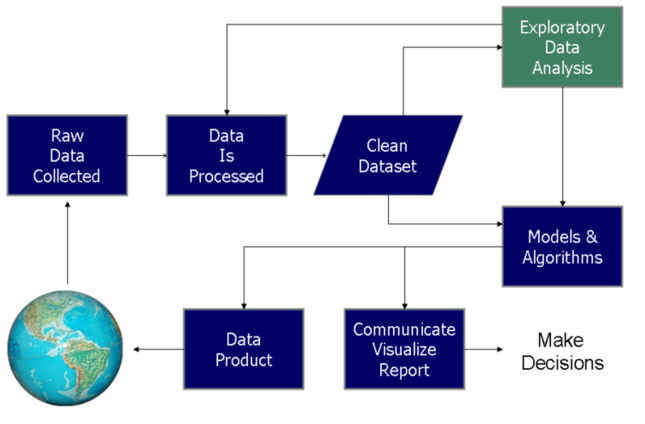
\includegraphics[width=1\textwidth]{Capture2}
\caption{The process of data science}
\end{figure}
\subsubsection{Data requirements}
{The data necessary as inputs to the analysis are specified based upon the requirements of those directing the analysis or customers who will use the finished product of the analysis. The general type of entity upon which the data will be collected is referred to as an experimental unit (e.g. a person or population of people). Specific variables regarding a population (e.g., age and income) may be specified and obtained. Data may be numerical or categorical (i.e., a text label for numbers).}
\subsubsection{Data collection}
{Data is collected from a variety of sources. The requirements may be communicated by analysts to custodians of the data, such as information technology personnel within an organization. The data may also be collected from sensors in the environment, such as traffic cameras, satellites, recording devices, etc. It may also be obtained through interviews, downloads from online sources, or reading documentation.}
\subsubsection{Data processing}
{The phases of the intelligence cycle used to convert raw information into actionable intelligence or knowledge are conceptually similar to the phases in data analysis.
Data initially obtained must be processed or organized for analysis. For instance, this may involve placing data into rows and columns in a table format for further analysis, such as within a spreadsheet or statistical software.}
\subsubsection{Data cleaning}
{Once processed and organized, the data may be incomplete, contain duplicates, or contain errors. The need for data cleaning will arise from problems in the way that data is entered and stored. Data cleaning is the process of preventing and correcting these errors. Common tasks include record matching, deduplication, and column segmentation. Such data problems can also be identified through a variety of analytical techniques. For example, with financial information, the totals for particular variables may be compared against separately published numbers believed to be reliable. Unusual amounts above or below pre-determined thresholds may also be reviewed. There are several types of data cleaning that depend on the type of data. Quantitative data methods for outlier detection can be used to get rid of likely incorrectly entered data. Textual data spellcheckers can be used to lessen the amount of mistyped words, but it is harder to tell if the words themselves are correct.}
\subsubsection{Exploratory data analysis}
{Once the data is cleaned, it can be analyzed. Analysts may apply a variety of techniques referred to as exploratory data analysis to begin understanding the messages contained in the data.The process of exploration may result in additional data cleaning or additional requests for data, so these activities may be iterative in nature. Descriptive statistics such as the average or median may be generated to help understand the data. Data visualization may also be used to examine the data in graphical format, to obtain additional insight regarding the messages within the data.}
\subsubsection{Modeling and algorithms}
{Mathematical formulas or models called algorithms may be applied to the data to identify relationships among the variables, such as correlation or causation. In general terms, models may be developed to evaluate a particular variable in the data based on other variable(s) in the data, with some residual error depending on model accuracy (i.e., Data = Model + Error).
Inferential statistics includes techniques to measure relationships between particular variables. For example, regression analysis may be used to model whether a change in advertising (independent variable X) explains the variation in sales (dependent variable Y). In mathematical terms, Y (sales) is a function of X (advertising). It may be described as Y = aX + b + error, where the model is designed such that a and b minimize the error when the model predicts Y for a given range of values of X. Analysts may attempt to build models that are descriptive of the data to simplify analysis and communicate results.}
\subsubsection{Data product}
{A data product is a computer application that takes data inputs and generates outputs, feeding them back into the environment. It may be based on a model or algorithm. An example is an application that analyzes data about customer purchasing history and recommends other purchases the customer might enjoy.}
\subsubsection{Communication}
{Data visualization is used to understand the results of a data analysis. Once the data is analyzed, it may be reported in many formats to the users of the analysis to support their requirements. The users may have feedback, which results in additional analysis. As such, much of the analytical cycle is iterative.When determining how to communicate the results, the analyst may consider data visualization techniques to help clearly and efficiently communicate the message to the audience. Data visualization uses information displays such as tables and charts to help communicate key messages contained in the data. Tables are helpful to a user who might lookup specific numbers, while charts (e.g., bar charts or line charts) may help explain the quantitative messages contained in the data.}
\subsection{Benefits of Data Analysis}
{The main benefits of data analysis are rather self-evident. How can someone improve their processes and identify problematic issues if they are not willing to look at the data? The answer, of course, is that they cannot make reliable improvements without data analysis. The key word here is “reliable!” Most people have a general idea about possible changes that “should” or “could” improve their processes. However, when it comes to these sorts of changes there is the inherent risk that the change does not have the desired result. There can also be unexpected consequences that impact some other aspect of that organization in a negative manner. Having said that, the following are just some of the benefits of proper data analysis:
\begin{itemize}
\item {Allows for the identification of important (and often mission-critical) trends}
\item {Helps businesses identify performance problems that require some sort of action Can be viewed in a visual manner, which leads to faster and better decisions}
\item {Better awareness regarding the habits of potential customers}
\item{It can provide a company with an edge over their competitors}
\end{itemize}
The process of evaluating data using analytical and logical reasoning to examine each component of the data provided. This form of analysis is just one of the many steps that must be completed when conducting a research experiment. Data from various sources is gathered, reviewed, and then analyzed to form some sort of finding or conclusion. There are a variety of specific data analysis method, some of which include data mining, text analytics, business intelligence, and data visualizations.}\\ \\
\textbf{\large Conclusion}\\ \\

{According to this chapter, we can classify our work as a quantitative data analysis project in which we aim to get some conclusion based on the data gathered, processed and visualized ,so lets treat now the data part in the next chapter called semantic technologies.}
\chapter{Semantic technologies}
\textbf{\large Introduction}\\ \\
{This chapter contains the basis of the semantic web .It presents also the well known Resource Description Framework and its query language SPARQL.}
\section{Semantic web}
\label{sec:sem}
\subsection{Overview}
{       The current web represents information using natural languages, graphics and multimedia objects which can be easily understood and processed by an average user. Some tasks on the web require combining data on the web from different sources e.g. travel and hotel information may come from different web sites when booking for a trip. Humans can merge this information and process them quite easily.\\
 However, machines can not combine such information and process it. Most of the Web’s content today is designed for humans to read, not for computer programs to manipulate meaningfully. Computers can adeptly parse Web pages for layout and routine processing – here a header, there a link to another page but in general, computers have no reliable way to process the semantics.
The Semantic Web will bring structure to the meaningful content of Web pages, creating an environment where software agents roaming from page to page can readily carry out sophisticated tasks for users.\\
The  Web of Data is not a separate Web but an extension of the current one, in which information is given well-defined meaning, better enabling computers and people to work in cooperation.
In addition, the semantic web  is a mesh of information linked up in such a way as to be easily processable by machines, on a global scale.\\
You can think of it as being an efficient way of representing data on the World Wide Web, or as a globally linked database.\\
The Semantic Web was thought up by Tim Berners-Lee, inventor of the WWW, URIs, HTTP, and HTML.\\
There is a dedicated team of people at the World Wide Web consortium (W3C) working to improve, extend and standardize the system, and many languages, publications, tools and so on have already been developed. \\
However, Semantic Web technologies are still very much in their infancies, and although the future of the project in general appears to be bright, there seems to be little consensus about the likely direction and characteristics of the early Semantic Web
      In addition to the classic “Web of documents” W3C is helping to build a technology stack to support a “Web of data,” the sort of data you find in databases.\\
The ultimate goal of the Web of data is to enable computers to do more useful work and to develop systems that can support trusted interactions over the network.\\
 The term “Semantic Web” refers to W3C’s vision of the Web of linked data. Semantic Web technologies enable people to create data stores on the Web, build vocabularies, and write rules for handling data.\\
Linked data are empowered by technologies such as RDF, SPARQL and OWL.}
\subsection{Semantic web architecture}
\begin{figure}[ht]
\centering
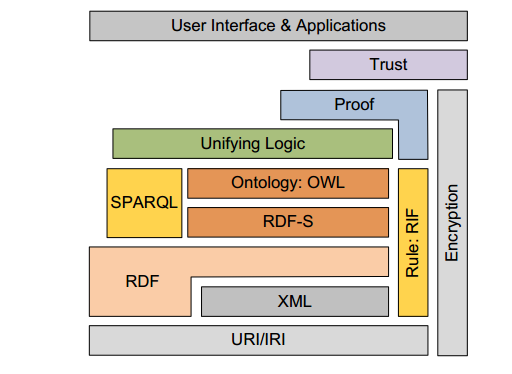
\includegraphics[width=1\textwidth]{Capture0}
\caption{Semantic web architecture}
\end{figure}

{  The first layer, URI and Unicode, follows the important features of the existing WWW. In fact , Unicode is a standard of encoding international character sets and it allows that all human languages can be used on the web using one standardized form.\\
 The Uniform Resource Identifier (URI) is a string of a standardized form that allows to uniquely identify resources such documents. \\
A subset of URI is Uniform Resource Locator (URL), which contains access mechanism and a (network) location of a document - such as http://www.example.org/. The usage of URI is important for a distributed internet system as it provides understandable identification of all resources.\\
 An international variant to URI is Internationalized Resource Identifier (IRI) that allows usage of Unicode characters in identifier and for which a mapping to URI is defined. \\
In the rest of this text, whenever URI is used, IRI can be used as well as a more general concept.\\
Extensible Markup Language (XML) layer with XML namespace and XML schema definitions makes sure that there is a common syntax used in the semantic web.\\
 XML is a general purpose markup language for documents containing structured information. \\
An XML document contains elements that can be nested and that may have attributes and content. XML namespaces allow to specify different markup vocabularies in one XML document.Moreover, XML schema serves for expressing schema of a particular set of XML documents.\\
A core data representation format for semantic web is Resource Description Framework (RDF) which is a framework for representing information about resources in a graph form. \\
It is based on triples subject-predicate-object that form graph of data. All data in the semantic web use RDF as the primary representation language. The normative syntax for serializing RDF is XML in the RDF/XML form.\\
 Formal semantics of RDF is defined as well.RDF itself serves as a description of a graph formed by triples.\\
Anyone can define vocabulary of terms used for more detailed description. To allow standardized description of taxonomies and other ontological constructs, a RDF Schema (RDFS) was created together with its formal semantics within RDF.\\
 RDFS can be used to describe taxonomies of classes and properties and use them to create lightweight ontologies.\\
More detailed ontologies can be created with Web Ontology Language OWL which  is a language derived from description logics, and offers more constructs over RDFS. It is syntactically embedded into RDF, so like RDFS, it provides additional standardized vocabulary. OWL comes in three species - OWL Lite for taxonomies and simple constrains, OWL DL for full description logic support, and OWL Full for maximum expressiveness and syntactic freedom of RDF. \\
Since OWL is based on description logic, it is not surprising that a formal semantics is defined for this language.RDFS and OWL have semantics defined and this semantics can be used for reasoning within ontologies and knowledge bases described using these languages. \\
To provide rules beyond the constructs available from these languages, rule languages are being standardized for the semantic web as well. Two standards are emerging - RIF and SWRL.\\
For querying RDF data as well as RDFS and OWL ontologies with knowledge bases, a Simple Protocol and RDF Query Language (SPARQL) is available.\\
 SPARQL is SQL-like language, but uses RDF triples and resources for both matching part of the query and for returning results of the query. \\
Since both RDFS and OWL are built on RDF, SPARQL can be used for querying ontologies and knowledge bases directly as well. SPARQL is not only query language, it is also a protocol for accessing RDF data.}
\section{Resource Description framework}
{The Resource Description Framework (RDF) is a language for representing information about resources in the World Wide Web. A resource is a physical or virtual entity, such as a person or an IP packet. RDF describes those resources in a subject-predicate-object structure.}
\subsection{Concept}
{RDF represents information by means of statements in a Subject-Predicate-Object structure:
\begin{itemize}
\item {Subject: a resource that is described by the statement}
\item {Predicate: a property of the resource that is described}
\item {Object: the value of the property of the resource that is described}
\end{itemize}
{Take for example the statement “Abderrahmen's emailAdress is abderrahmen.sdiri@supcom.tn”. The parts are:
\begin{itemize}
\item {Subject:Abderrahmen }
\item {Predicate:emailAdress}
\item {Object: abderrahmen.sdiri@supcom.tn}
\end{itemize}
{Since RDF is meant to be machine-processable, evey resource has to be unique to avoid confusion. The Web offers URI references to deal with this problem. Subjects and predicates are resources, and thus are to be represented by a URI reference. Objects can be resources, though they also can be a literal, which is a non-decomposable object, like a string or a number}
\subsection{Representation}
{RDF has in fact an inherent graph based structure, which can be serialized using turte, RDF/XML and others. The next paragraphs introduce representations for a group of statements. Forsome representations, an example is given for “Abderrahmen is called Abderrahmen S and is 24 years old. Ahmed is his friend. The FOAF  ontology is used to describe these statements. Note that since URIs can be long, they can be shortened in a more clear notation, using prefixes. Therefore a URI reference is split up in a namespace and local name.
This namespace is represented by a prefix. The notation is shortened as  \verb!prefix:local_name!. For instance,\url{ http://xmlns.com/foaf/0.1/name}  is  equivalent to \verb!foaf:name!, using foaf as a prefix for  \url{http://xmlns.com/foaf/0.1/}.}
\subsection{Graph model notation}
{RDF statements lend themselves easily to be represented as a graph. Subjects and objects are the equivalent of the nodes and predicates are labeled edges. Conceptually this means that a subject is connected to an object by means of a predicate. The following graph is the
representation of the earlier given example. Note that every resource, used as a subject or object, is unique; per resource only one node exists.
\begin{figure}[ht]
\centering
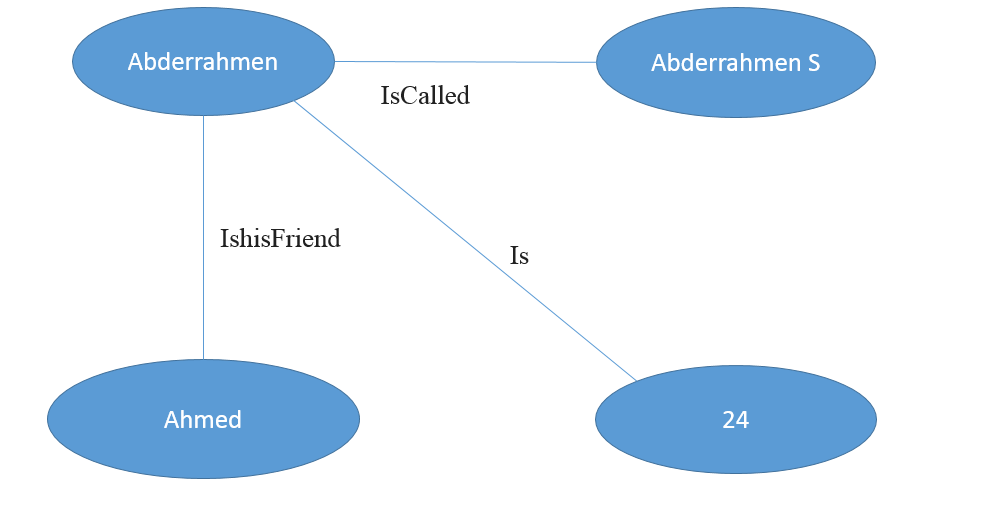
\includegraphics[width=1\textwidth]{Capture20}
\caption{Graph Representation}
\end{figure}
}
\subsection{RDF Turtle}
{Turtle (Terse RDF Triple Language) is a format for expressing data in the Resource Description Framework (RDF) data model with a syntax similar to SPARQL. RDF, in turn, represents information using "triples", each of which consists of a subject, a predicate, and an object. Each of those items is expressed as a Web URI.Turtle provides a way to group three URIs to make a triple, and provides ways to abbreviate such information, for example by factoring out common portions of URIs. For example:\\
\url{<http://example.org/person/Abderrahmen>} \url{<http://example.org/relation/student>}  \url{<http://example.org/engineeringSchools/SUP'COM>} .}
\subsection{RDF XML}
{RDF uses XML as a structure to guarantee the machine-pro cess ability and interchangeability.XML is a markup language that allows creating a custom document format. Hence, RDF/XMLis a representation for state ments.\\
RDF identifies things using Web identifiers (URIs), and describes resources with properties and property values.\\
Explanation of Resource, Property, and Property value:
A Resource is anything that can have a URI, such as\url{< http://example.org/person/Abderrahmen>}.
A Property is a Resource that has a name, such as \url {http://example.org/relation/student}
A Property value is the value of a Property, such as \url {<http://example.org/engineeringSchools/SUP’ COM>}\\
The following RDF document could describe the resource \url {http://example.org/person/Abderrahmen}:\\
\begin{figure}[ht]
\centering
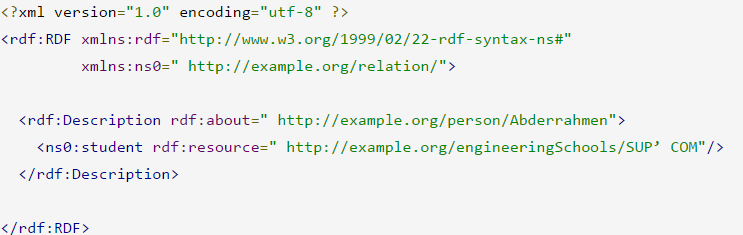
\includegraphics[width=1\textwidth]{Capture21}
\caption{RDF/XML Representation}
\end{figure}
 }
\subsection {RDFS}
{RDF is used to structure and represent statements about resources. It does not specify what the meaning of those statements is. In other words, the statements lack semantics. RDFS (RDF Schema) deals with that problem and offers the possibility to create vocabularies, also written in RDF. Therefore RDFS uses the notion of classes and properties.\\
The vocabularies describe the semantics of these classes and properties. By using them in RDF, reuse of semantics is possible. RDFS has many other features, including domain and range definition for a property.\\
The next figure is an example of a simple vocabulary of an animal. Pet has two subclasses Mammal and Bird. Dog is a subclass of Mammal. Due to the subclassing, all mammels (including dogs) and birds also have the property name, which is defined for Pet and is a literal}
\begin{figure}[ht]
\centering
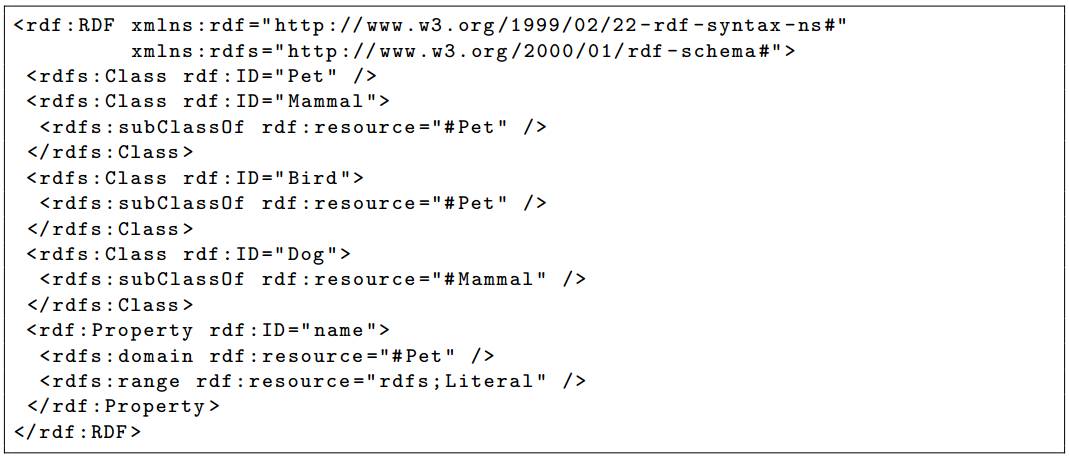
\includegraphics[width=1\textwidth]{Capture4}
\caption{RDF Schema Example}
\end{figure}
{Therefore, RDF Schema language, provides the syntax for defining the general RDF vocabulary as well as domain-specific vocabularies. RDFS is built on top of RDF, so that RDFS data is also valid RDF data.  RDFS introduces the concepts of classes and their properties.  In particular, RDFS allows for specifying classification and generalisation hierarchies for both metadata properties and values. Using RDFS it is possible to distinguish between RDF instance data and its schema.}
\section{OWL}
{ OWL  (Web Ontology Language) is, like RDFS, a language to define vocabularies. It facilitates greater machine interpretability by providing more vocabulary, thus is more expressive thanRDFS. OWL adds, among others, cardinality, relations between classes and more properties.
OWL comes in three flavours, which are ordered by increasing expressiveness:
\begin{itemize}
\item {OWL Lite only defines a classification hierarchy and simple cardinality constraints. }
\item { OWL DL supports maximum expressiveness and guarantees computational completeness
(computable). Every computation also is decidable (finishes in a finite time).}
\item { OWL Full handles every aspect of OWL DL without any computational guarantees.}
\end{itemize}
While it is possible to define your own vocabularies, reusing existing ones facilitates understandability of your data. A commmonly used vocabulary to describe persons is Friend-Of-A-Friend (FOAF).\\
Thus ,ontologies are used to capture knowledge about some domain of interest. An ontology describes the concepts in the domain and also the relationships that hold between those concepts. Different ontology languages provide different facilities.\\
 The most recent development in standard ontology languages is OWL from the World Wide Web Consortium (W3C) . Like Protégé, OWL makes it possible to describe concepts but it also provides new facilities.\\
 It has a richer set of operators - e.g. intersection, union and negation. It is based on a different logical model which makes it possible for concepts to be defined as well as described. Complex concepts can therefore be built up in definitions out of simpler concepts. Furthermore, the logical model allows the use of a reasoner which can check whether or not all of the statements and definitions in the ontology are mutually consistent and can also recognise which concepts fit under which definitions. The reasoner can therefore help to maintain the hierarchy correctly.\\
 This is particularly useful when dealing with cases where classes can have more than one parent.}
\section{SPARQL and SPARQL Endpoints}
SPARQL (SPARQL Protocol and RDF Query Language) is a query language for RDF. It also anchors the protocol which clients use to access a SPARQL endpoint.
\subsection{Syntax}
{In this section, the basic syntax of the SELECT feature is highlighted. However, many other
query forms are supported by SPARQL (CONSTRUCT, ASK and DESCRIBE), but they are not described in detail, as they are not used in this project. SPARQL does not support commands that alter data, such as UPDATE, etc.\\
The next figure wants to retrieve the names of all persons in the dataset. The SELECT keyword asks the endpoint to bind every matching RDF resource or literal to the defined variables.
The WHERE clausule restricts the possible bindings by making a subset of the dataset, based on the statements that are specified. Variables are represented by the prefix ?. Literals are placed between double quotes. The PREFIX command implements the concept of shortened
notation of resources. The query wants to retrieve the names of all persons in the dataset that know another person. The name of that person is also returned.}
\begin{figure}[ht]
\centering
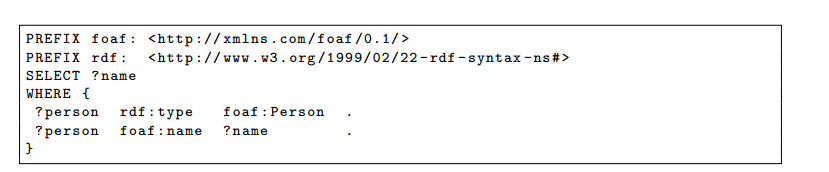
\includegraphics[width=1\textwidth]{Capture5}
\caption{SPARQL SELECT query}
\end{figure}
\subsection{Working of SPARQL}
{The results of a SPARQL query depend on the conditions specified in the WHERE-clause, since they filter the queried RDF dataset. As stated before, RDF statements have an inherent graph based structure. This also applies for a WHERE-clause, as that is a collection of statements. Each graph contains one or more patterns. There are various types of such graph patterns, proportional to the complexity of the WHERE-clause.In order to filter a dataset, SPARQL uses the notion of graph patterns
to apply graph pattern matching between the dataset’s graph and the graph of its WHEREclause. This approach is completely different from SQL’s, which acts in a procedural way for querying relational datasets, without an implicit join feature. That is, joins have to be
specified explicitly in order to combine data, whereas in SPARQL, this is already provided by the structure of RDF}
\subsection{SPARQL endpoints}
{SPARQL endpoints are web applications that offer an interface to an RDF dataset in the form of a plain HTTP GET-request. The SPARQL protocol is hidden for the end users. There exist many SPARQL endpoints on the Web . Users can set up their own endpoint using some
software like OpenLink Virtuoso  or Apache Jena Fuseki. In this project, Fuseki is used to set up multiple sources with distributed data}\\ \\
\textbf{\large Conclusion}\\ \\

{In this chapter we have defined the most important technologies of the web of data.Those technologies will be be used in the practical work of this project  and we will return to the basic concepts in every step of the transformation of our raw data to  into linked data  and finally  we will touch the importance of SPARQL for retreiving useful information in the  last chapter of this report.}

\chapter{Linking open data project}
\textbf{\large Introduction}\\ \\

{Linked data is about using the web to connect data that wasn't previously linked.In this chapter , we will sit the principles of linked data  , its application  and then we will focus on the open linked data cloud which is a very important project for linking data on the web.}
\section{Open Data}
{In this project the used data are called Open Data. Even though the term Open Data is currently in frequent use, there is no commonly agreed definition. We will use the one provided by the Open Knowledge Definition (OKD) project.\\
OKD considers data as any kind of content from “sonnets to statistics, genes to geodata”.\\
 According to the OKD definition, data is open “if anyone is free to use, reuse, and redistribute it - subject only, at most, to the requirement to attribute and sharealike”.\\
 This definition considers three aspects of data openness: social, technological and legal. Social openness means that the data must be accessible as a whole, and not only few items of it at a time (e.g., by downloading).\\
 By technological openness OKD considers absence of any technological obstacles to access and reuse the data (e.g., no,access control and open formats). Legal openness is established by open data licenses.\\
\textbf{Open Data licensing:} Open licenses meet the requirements of Open Data and grant permissions to access, reuse and redistribute data with few or no restrictions. In order to enable people to use the data on the Web on a secure legal basis, one needs to
explicitly state which license applies to your data. It is important to apply open data licenses simply for the sake of clarity. \\
Without a license it is not clear if the data can be used, reused and distributed by others. Examples of open licenses include Public Domain Dedication and License (PDDL) and Attribution License by the Open Data Commons project, the GNU Free Documentation License and the licenses prepared by the Creative Commons Attribution project, such as Creative Commons AttributionShare-Alike (cc-by-sa).\\
\textbf{Open data sets:} There are various interesting open data sets available on the Web. A well-known example of open data is Wikipedia. Most of the Wikipedia’s text and many of its images are under open licenses. Other examples of open data are Wikibooks, Geonames, MusicBrainz, WordNet and the DBLP bibliography. \\
Google Maps is an example of data that is not open, since the geodata is currently proprietary (copyrighted or protected by DB rights).\\
In general, Open Data can come from anywhere. One of the biggest source of Open Data is the government domain. Open Government Data is a global movement of governments starting to open their information from public sector.
The pioneers were the governments of the U.S.  and the U.K, and many more governments have already joined the movement, including Australia, Netherlands, Spain, Austria, Denmark}
\section{Linked Data}
{The term Linked Data was coined by Tim Berners-Lee in 2006 in his design note . He outlined a set of recommendations, referred to as Linked Data principles, on how to complement the current Web of human-oriented documents with a Web of machineenabled data. \\
Tim Berners-Lee proposed to apply the same ideas that are successfully used for making the current Web, to publish and interlink data in such a way that machines can also process it and extract its meaning, i.e., build a Web of Data.\\
\subsection{The Linked Data principles}
{The Linked Data principles in its original reading are as follows :}
\begin{enumerate}
\item{Use URIs as names for things}
\item{Use HTTP URIs so that people can look up those names}
\item{When someone looks up a URI, provide useful information, using the standards (RDF,SPARQL)}
\item{Include links to other URIs. so that they can discover more things}
\end{enumerate}
\textbf{The Linked Data principles in a nutshell:}  The classic Web provides humans with data. It can be any kind of data, e.g., air temperature, somebody’s personal profile, official government reports, etc. The data is represented in the form of documents (e.g.,
HTML Web pages). Documents can be processed by machines that can “understand” the structure of the documents (e.g., paragraphs, titles, tables, etc.) and present them in a more convenient way for humans to read and comprehend the data carried out by the documents.\\ However, the meaning of the data is mostly given as a plain text and hidden from the machines. \\
It is hard for software applications to extract semantics from HTML pages. To allow machines to “understand” the meaning of the data, we need to be able to describe not only the structure of the documents, but the data itself. \\
At its most basic, data is made up of any kind of things that exists in the world, i.e., real-world objects (e.g., people, countries, building, etc.) or abstract concepts (e.g., air temperature, the fact of knowing somebody, etc.). Thus, the Web of Data extends the scope of the traditional Web from documents to encompass real-world objects and abstract concepts.\\
The first and second Linked Data principles define a mechanism to name any thing that exists in the world using the existing Web standards, such as URI and HTTP , and make them accessible
on the Web. For example, by using the Linked Data principles one can give a name the concept of city of Lisbon and publish it on the Web. Noting that the city of Lisbon and its homepage are not the same concept. For this reason they must be named with two
different URIs.\\
The conventional Web has its standard way to describe documents on the Web, i.e., HTML is used to create Web pages. The third Linked Data principle recommends to use the Resource Description Framework (RDF) to describe things in the world in a machine-redable manner .\\
 In RDF one can provide descriptions of real-world concepts in the form of sentences. For example, one may describe the Lisbon city as follows: Lisbon is the capital of Portugal; Lisbon has population 545,245 people, etc.
Finally, links are an integral part of a Web. Documents on the classic Web are connected by means of the hypertext links.\\
 Similarly, the fourth Linked Data principle claims to connect data on the Web by setting links to data from other data sources.
Links on the Web of Data are defined using RDF and referred to as RDF links.\\
 Unlike the hypertext links, the links on the Web of Data not only connect two pieces of data together, they also provide semantics for this connection.\\
 The RDF links look like sentences as well, just involve concepts that were defined by different people. For example, if you define the concept of the city of Lisbon and discover that somebody else in another dataset defined the concept of Portugal, then the following link can be set Lisbon is the capital of Portugal (where Portugal is the concept from that external dataset). Thus, you can connect your data with this external dataset.\\
\textbf{Linked Data vs Linked Open Data} The fact that Linked Data is defined in a personal note of Tim Berners-Lee and is not formally endorsed by W3C contributes to the ambiguity of the definition of the concept of Linked Data. The discussions regarding this
topic generally come down to which technology is used to represent data.\\
 Some people argue that RDF is integral to Linked Data, others suggest that, while it may be desirable, use of RDF is optional rather than mandatory. Some reserve the capitalized term
Linked Data for data that is based on RDF, preferring lower case linked data, or linkable data, for data that uses other technologies.\\
 In our work we will use the term Linked Data
to refer to data published on the Web in accordance with the Linked Data principles. \\
We will also stick to the most common opinion that RDF is a standard for representing Linked Data. When we want to emphasize that the Linked Data principles were
applied to Open Data we will use the term Linked Open Data.}
\section{Linking Open Data project}
{The LOD project began in 2007 with the support and sponsorship of the W3C Semantic Web Education and Outreach Group (SWEO) . The goal of the project is to bootstrap the Web of Data. Initially, the project was driven mainly by researchers
in university research labs and Web enthusiasts, whose aim was to identify Open Data and serve it as Linked Data on the Web. Since 2007 the project has grown considerably due to the involvement from large organizations from different domains. According to the latest statistics of September 2011, the scope of the Linking Open Data project included 295 datasets.\\
\begin{figure}[h!]
\centering
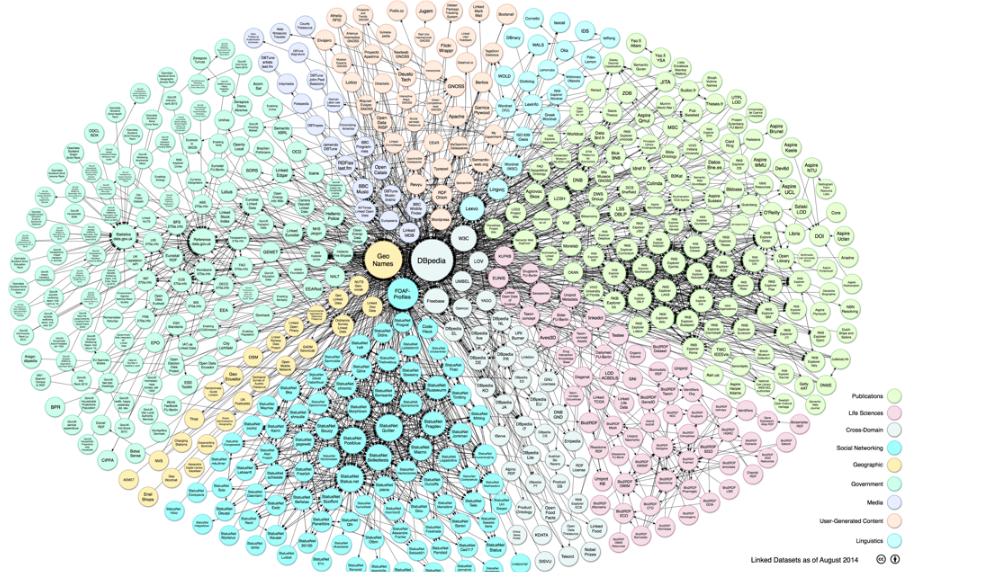
\includegraphics[width=1\textwidth]{Capture6}
\caption{LOD cloud diagram as of September 2014}
\end{figure}
The next Figure demonstrates the range and scale of the Web of Data originating from the LOD project.
Each node in the LOD cloud diagram represents a distinct Linked Data set. The arcs indicate the connections between datasets. \\
The heavier the arcs are, the bigger number of links exist. Bidirectional arcs represent links in both directions. For keeping the
LOD cloud diagram up to date, the Linking Open Data community effort maintains acatalog of known Linked Data sources, the LOD Cloud Data Catalog }
\section{The LOD project activities}
{The next step of promoting Linked Data concerns demonstration how Linked Open Data can actually be used. The Linked Data standards represent the data in a structured machine-readable way with explicitly defined semantics.\\
 This gives new opportunities to work with data. Compare, for example, the way the number 2.3 is represented in an xls file and as Linked Data. \\
In xls this number is not of a huge value for machines, they operate with it as with another cell, without differentiating it from the number 3.1 for example. With Linked Data we can provide a meaning to these numbers. For example, The number 2.3 is the inflation rate in Portugal in 2005, when the president of Portugal was Jorge Sampaio, from the Socialist Party. The number 3.1 is the inflation rate in 2006, when the president Anibal Cavaco Silva from the Social Democratic Party was elected.\\
 Now machines can use these numbers to analyse inflation rate in relation to the political situation in the country. \\
The Web of Data contains a big collections of such structured machine-readable data interlinked to form a single global informational space. We can use the Web of Data to connect disparate data sources on the Web and develop new kinds of applications that operate upon such data, so called Linked Data driven Web applications.\\
 As Linked Data is a relatively novel technology, the existing applications are mostly prototypes and will likely undergo significant evolution as lessons are learnt from their development and deployment. Nevertheless, they already give an idea of what will be possible in the future. The present Linked Data driven applications can be classified into generic applications, such as Linked Data browsers and search engines, and domain specific applications that cover the needs of specific user communities.}
\subsection{Linked Data browsers}
{In the classical Web of documents, browsers allow users to navigate between HTML pages by following untyped hypertext links, that can be understood by humans but are meaningless for machines, and, thus, can not be used to assist people in finding information and “guide” them through the Web in a smarter way.\\
 The Linked Data browsers are Web applications that provides interactive support for navigating through or exploring Linked Data. Examples of LD browsers include the LinkSailor , Tabulator , Marbles and URI Burner. They can process
the semantic links established between different data sources and facilitate users in exploring the Web of Data.\\
 For example, when a user is looking for the description of the city of Lisbon in DBpedia, Linked Data browsers can interpret the data available about Lisbon and present it nicely using conventional data presentation methods.\\
Thus, the browsers can “understand” that Lisbon is a city and represent it on a map, as well as other notable locations in the city such as theatres, castles, shops, etc., can be “recognized” by the browsers as having geographical characteristics and represented on the map. Tabulator and Marbles can also merge data about the same concept from different data sources.\\
They can discover that there are other data sources on the Web that also describe Lisbon, combine their data with the DBpedia data and present the aggregated view to the user.}
\subsection{Linked Data search engines}
{The Linked Data search engines also take advantage of the ability of machines to process and extract the meaning of information on the Web of Data. \\
The existing LD search engines provide richer interaction capabilities to a user and ensure more accurate search results, than classic search engines with a simple keyword-based search implemented. For example, DBpedia implements the faceted search paradigm  that allows users to filter search results according to specific criteria (facets), e.g., people who were born in a certain country or who have a specific profession.\\
 Thus, if a user searches for information about Armstrong, the bicyclist, the results can be narrowed to contain only data relevant to bicyclists, excluding those with data about Armstrong, the astronaut, or Armstrong, the jazzman, or other Armstrongs who were not outstanding bicyclists. \\
While DBpedia implements an enhanced search over the DBpedia dataset together with information from interlinked datasets such as Geonames, Freebase and DBLP bibliography, the Falcons search engine provides the same functionality at a Web scale
\begin{figure}[h!]
\centering
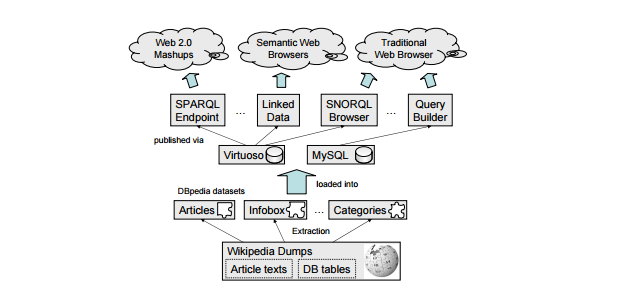
\includegraphics[width=1\textwidth]{Capture22}
\caption{Overview of the DBpedia components.}
\end{figure}

}
\subsection{Domain specific Linked Data applications}
{Domain specific Linked Data driven applications are those that reuse content of existing LODsets to fulfil different purposes. Numerous examples of such applications exist.\\
 The U.K. and U.S. governments are among the key institutions that have recognised the advantages in converting legacy data stores into Linked Data and making explicit links between these heterogeneous data sources. One direct benefit of Linked Data is richer government transparency: citizens can now participate in collaborative government data access, including “mashing up” distributed government data from different agencies, discovering interesting patterns, customizing applications, and providing feedback to enhance the quality of published government data.\\
 The Tetherless World Constellation (TWC)  investigates the role of Linked Data in producing, enhancing and utilising government data published on data.gov. For this, TWC develops visualisations and mashups of different government data, including financial data,
spending, energy usage and public healthcare. Their works for consuming Linked government data demonstrate how the value of the data is increased in combination with other datasets. For example, one application utilise the U.S. government data spending on fire fighting to integrate it with data from DBpedia about number of fires and burned area in different years.\\
 The application shows correlations between the government spending and the the actual fires. Another example combines the smokerrates statistics with data about population and cigarette taxes5. More works done by TWC can be found in.\\
The U.K. government gave rise to plenty of mashups and visualisations that show immediate benefits of the LD standards for citizens. Among them are applications that provide information about local services, help managing finance and environmental issues. For example, the “Walkonomics” application rates and maps the pedestrian friendliness of streets and urban areas combining government data with real people reviews. \\
It allows to check a street by a post code and helps to understand how walkable it is. Another example is the “BUSit London” application that reuses information about London buses and allows to plan a bus journey with several changes by indicating which buses to take, where to catch them and where to change.\\
 An interesting interactive visualisation of the U.K. government spending is developed by the Open Knowledge Foundation . \\
“Where Does My Money Go?”represents spending by area and helps to understand where the money of the UK taxpayers’ goes.
BBC is utilising the benefits of Linked Data as means for storing and sharing news. The BBC Programmes site  reuses information from other LODsets (e.g., DBpedia
and Freebase) to identify and link semantically related information owned by the BBC to increase usability of their web pages and other applications that make use of it.\\
The BBC Music site  is enriched with artists information from MusicBrainz  and artists’ biographies fetched from DBpedia to compose introductory texts.
Talis Aspire  is a Linked Data driven application that helps educators to create and manage lists of learning resources, e.g., books, journal articles, Web pages.\\
 Users interact with the application via a conventional Web interface, while the data they create is stored as Linked Data. Aspire then uses the Linked Data principles to connect the learning resources with related data elsewhere on the Web and enrich the range of material available to support the educational process.\\
 This resource list management system is currently used by thousands of students at the University of Plymouth and the University of Sussex . Another interesting application that reuses the DBpedia data is a generic reviewing and rating site, Revyu 9. For example, when a film is reviewed on Revyu, the site attempts to provide more information about the film (e.g., the director’s name and the film poster) by reusing the data from DBpedia.\\
An interesting mobile application was developed upon the DBpedia dataset, DB-pedia Mobile . This application helps tourists to explore a city by identifying their location based on the current GPS signal of the mobile device and rendering a map with indications of nearby interesting places.\\
One of the examples of Linked Data driven applications in the life science domain is the NCBO Resource Index . It relies on LOD from different biomedical datasets on the Web of Data and supports researchers in exploring them. \\
Zemanta  is a content recommendation tool that reuses data from DBpedia and Freebase in order to help users to better organize their blogging activities.\\
It suggests relevant links, articles or images while users write their blogs to make them more interesting and attractive for readers. Google uses Linked Data describing people, products, businesses, organizations, reviews, recipes and events in its search results to provide them in the form of rich snippets .\\
 It also uses the extracted Linked Data to directly answer simple factual questions such as the birth date or place of somebody. Google answers such queries not only with a list of relevant links, but it provides the actual answer.}\\ \\
\textbf{\large Conclusion}\\ \\
{The most visible example of adoption and application of the Linked Data principles has been the Linking Open Data project which is presented in this chapter.The following chapter will treat the visualization approches of the linked data in order to make our analysis. }

\chapter{Linked Open Data Visualization }
\textbf{\large Introduction}\\ \\
{The visualization of linked data is the key of making our data analysis in this project.We will present in this chapter the different approches of  linked data visualization which will help us to choose the  more efficient visualization technique to use in this project. }
\section{Linked Data Visualization and Exploration}
{The amount of semantic data available on the Web has increased dramatically, especially thanks to initiatives like Linked Open Data (LOD)  already presented in the previous chapter. \\
The potential of this vast amount of data is enormous but in most cases it is very difficult and cumbersome for users to visualize, explore and use this data, especially for lay-users  without experience with Semantic Web technologies.\\
Visualizing and interacting with Linked Data is an issue that has been recognized from the beginning of the Semantic Web .\\
Applying information visualization techniques to the Semantic Web helps users to explore large amounts of data and interact with them.\\
The main objectives of information visualization are to transform and present data into a visual representation, in such a way that users can obtain a better understanding of the data.\\
 Visualizations are useful for obtaining an overview of the datasets, their main types, properties and the relationships between them.\\
Compared to prior information visualization strategies, we have a unique opportunity on the Data Web.\\
 The unified RDF data model being prevalent on the Data Web enables us to bind data to visualizations in an unforeseen and dynamic way.\\
 An information visualization technique requires certain data structures to be present. When we can derive and generate these data structures automatically from reused vocabularies or semantic representations, we are able to realize a largely automatic visualization workflow.\\ Ultimately, we aim to realize an ecosystem of data extractions and visualizations, which can be bound together in a dynamic and unforeseen way.\\
 This will enable users to explore datasets even if the publisher of the data does not provide any exploration or visualization means.
Most existing work related to visualizing RDF is focused on concrete domains and concrete datatypes. The Linked Data Visualization Model (LDVM)  allows to connect different datasets with different visualizations in a dynamic way. LDVM balances between flexibility of visualization options and efficiency of implementation or configuration. }
\section{Motivating use cases}
\subsubsection{What Can I See in the Given Data?}
{The first use case is to show possible visualizations of datavin a given dataset. The dataset must be given in an easy way - using either a link to an RDF dump or using direct RDF file upload, or using a link to a SPARQL endpoint that
contains the data. The result should be a list of possible visualizations that could be meaningful for the dataset.\\
 When the user clicks on a possible visualization, he should see his data visualized by the selected technique, e.g. on a map,vusing a hierarchy visualizer, etc. This use case has several motivations.\\
Firstly, one should be able to quickly sample a previously unknown dataset that may be potentially useful based on its textual description such as the one on http:v//datahub.io. \\
 Another motivation for this use case is the need to be able to quickly and easily show someone what can be done with his data in RDF. In addition, this use case can help Linked Data experts even during the process of Linked Data creation which usually happens in iterations. In the first iteration of creating Linked Data an expert usually writes a transformation of some basic information about entities in the source data such as their names and types.\\
Then he reviews the created RDF data, selects another portion of the source data, amends his transformation, executes it and again observes the resulting, more detailed RDF data. He repeats this process until all of the source data, or at least the desired parts, is transformed to RDF.\\
 The iterations can be fast, when the expert knows the source data and the desired RDF form well, or they can be slow, when for example the expert shows the result of each iteration to a customer and discusses what part of the source data is he going to transform
next. \\
Either way, it would be better to have a visualization accompanying the data in each iteration, which would show how the data gets better and more detailed. Also, trying to visualize the resulting data provides additional means of
validation of the transformation, e.g. when it is entities on a map, it is always better to see the result on a map than just an RDF text file.\\
On the other hand, the visualization method needs to be quick and easy and not custom made for the data, because the data between iterations is only temporary as it lasts only until it gets improved in the next iteration. However, this is made possible by the Linked Data vocabulary reuse principle, all we need is a library of components supporting standard vocabularies and usage of the vocabularies in the data, which is a well known best practice.\\
 Finally, when developing advanced visualizations, the designer can start with the automatically offered one and refine it instead of starting from scratch.
An example of this use case is that when a dataset containing a hierarchy is provided, then a visualization using a hierarchy visualizer should be offered and it should display some meaningful data from the source dataset.\\
 To be specific, we will show this use case on a dataset that contains a hierarchy or regional units ranging from individual address points to the whole country.
\subsubsection{What Can I Combine My Data With To See More}
{The second use case is to show which additional visualizations of the input data can be used when the data is simply linked to another dataset. One motivation of this use case is to visually prove the value of linking by showing the additional visualization options gained by it.\\ Another motivation is the expert in a modern company that has its internal linked data and wants to see the improvement gained by linking it to the public LOD cloud. For this use case the user should be able to provide his data easily as in the previous
use case. This time he is interested in seeing which additional visualizations of his data he can use when he linked his data to another dataset.\\ The result should again be a list of possible visualizations which, however, use not only the input
dataset, but also some other to achieve a better visualization. For example, a dataset with addresses of public institutions, linked to a geocoded dataset of all addresses yields a map visualization with no additional effort.}
\subsubsection{What Data Can I Visualize Like This}
{The third use case is a reverse one compared to the previous two. It is to show datasets or their combinations which can be visualized using a selected visualizer.\\ The motivation for this use case is that the user sees a visualization that he
likes and he wants to prepare his data so that it is compatible with the visualization. For that he wants to see which other datasets possibly combined with some transformations use this visualization. \\ For this use case the user selects a visualization and he should get a list of data sets possibly with transformations which can be visualized by the selected visualizer. For example, the user selects a map visualizer and he should see that a dataset with a list of cities can be visualized this way.}
\section{ Actual approaches to visualising LOD}
\subsection{CODE Visualization Wizard}
{Within the EU-funded research project CODE3, the Vis Wizard tool  envisages a visualization platform for all the research publications data extracted due to the project’s efforts.
To publish research data on the LOD cloud, CODE relies on the RDF Data Cube Vocabulary (DCV) , a W3C standard developed to represent statistical data as RDF. Document parser’s output is mapped to the DCV as a collection of observations consisting in a set
of dimensions and measures.
\begin{figure}[h!]
\centering
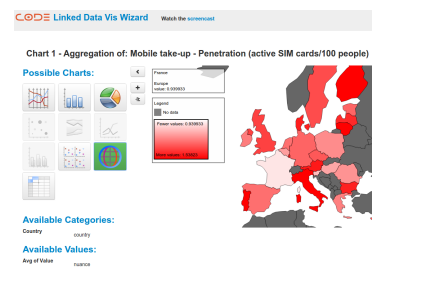
\includegraphics[width=1\textwidth]{Capture9}
\caption{CODE Linked Data Vis Wizard, with the map selected as the representation to display data, among other options}
\end{figure}
Once data is loaded in the system, Vis Wizard highlights the visual representations that can fit the selected data as shown in Figure4.1, depending on its nature. For example, if planar data are found the users will be able to draw a map, disabling the selector otherwise.\\This
recommendations can be improved by implementing new generators, well-defined interfaces with the ability to map data to new visualizations when plugged to the Vis Wizard.\\
 Lay users can interact with the data by adding and removing dimensions, and changing the visual components they are referenced to.\\ This opens new opportunities to customize the way data is presented.\\
Finally, using mindmeister’s Mind Mapping software , a history of the performed actions, applied filters and generated visualizations can be observed, in order to make data analysis processes reproducible.}
\subsection{LDVizWiz}
{With the goal of providing general purpose visualizations of any SPARQL endpoint, LDVizWiz  inspects the features of the dataset in order to understand the underlying data and detect categories.
Based on the classification provided by Shneiderman, LDVizWiz performs ASK queries to categorise data in one of the following classes: Geography, Temporal, Event, Agent/Person, Organization, Statistics and Knowledge.
\begin{figure}[h!]
\centering
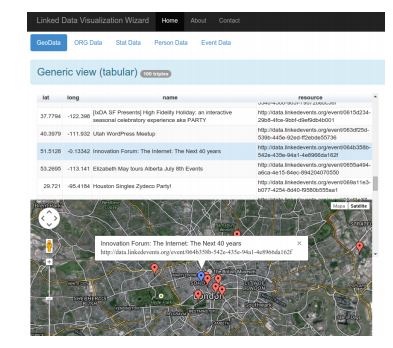
\includegraphics[width=1\textwidth]{Capture10}
\caption{LDVizWiz’s display or detected GeoData}
\end{figure}
Even though some of the categories have a direct mapping to Shneiderman’s taxonomy and certain vocabularies, for example, geography ↔ planar data as seen in Figure4.2, temporal data and knowledge information ↔ hierarchical, others such as Agent/Person
or Organization are related to whole ontology class instances.\\
 This non-datatype based approach loses some of the advantages provided by best practices and lessons learned from the data visualization field, although class-category template filling exhibits a more
robust performance if the schema is known beforehand. The biggest drawback is the need to adapt and extend the ASK queries to new vocabularies whenever they are detected.}
\subsection{LODVizSuite \& ResXplorer}
{Researchers from the iMinds Digital Research Centre5 designed, implemented and evaluated an interactive visual workflow to explore LOD. The workflow uses EDA techniques to guide users through the exploratory stage, and Exploratory Search  concepts
to ease data querying. EDA is allowed through narrowing the dataset from high level group overviews towards their details. Providing an overview first, the dataset reveals its underlying structure and the internal connections as the users
explore deeper in the content. The tool designed for this purpose is named LODVizSuite .
Exploratory Search consists on broadening a coordinated view (output of the narrowing phase). This set of actions is highly focused on leading to other datasets through relationships, if they are considered relevant enough. Broadening is provided by the ResXplorer tool .
\begin{figure}[h!]
\centering
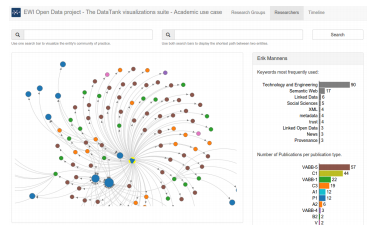
\includegraphics[width=1\textwidth]{Capture11}
\caption{LODVizSuite rendering of a research co-authorship network using a force directed layout}
\end{figure} }
{For the workflow’s implementation, the Research Information Linked Open Data (RILOD) dataset is used, an integration of heterogeneous sources related with research and investigation within the region of Flanders. Figure 4.3 shows the connections between researchers, with a sidebar displaying the amount of topics covered by the selected author in the graph. The data contained within the dataset is enriched with Digital Bibliography and Library Project (DBLP)6 using ResXplorer.}
\subsection{LODVisualization}
{LODVisualization is a tool based on the LDVM (Linked Data Visualization Model)  that allows to connect different data sources in a dynamic way using different visual representations. LODVisualization adopts the Data State Reference Model (DRM) as
a conceptual framework, implementing it according to the features of LOD as exhibited in Figure 4.4 .
\begin{figure}[h!]
\centering
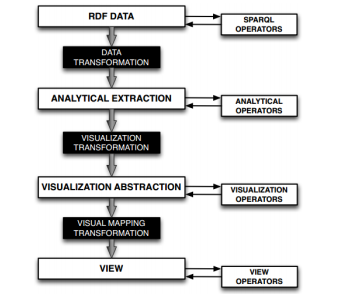
\includegraphics[width=1\textwidth]{Capture12}
\caption{LDVM’s implementation of Ed Chi’s DRM}
\end{figure}
The tool implements the Overview task proposed by Shneiderman, generating visual representations about the hierarchy of classes and properties defined in a SPARQL endpoint graph. Users can also consult the shared properties between two classes, or those instances with the highest in/out-degrees, i.e., resources of a given class with the highest number of outgoing and incoming links.\\
However, instances referring to the same entity are not disambiguated and are displayed iteratively.
LODVisualization can draw treemaps, tables and bar charts with the extracted data from any SPARQL endpoint, without the need of adapting to a certain set of domains. Still, it does not perform the rest of tasks defined by Shneiderman.}
\subsection{Payola}
{Payola  provides a refined implementation of the LDVM, to generate visualizations for the Czech LOD cloud, a set of public datasets with relevant data for Czechoslovakians, such as public inspections and sanctions depicted in Figure 4.5 . Users are able to connect to a SPARQL endpoint or upload a RDF file, performing different analysis over the data and visualising them on a web browser, thanks to the implementation of LDVM pipelines. Tech-users can also improve the SPARQL queries and add plugins to Payola in order to
get a more refined outcome of the analysis.
\begin{figure}[h!]
\centering
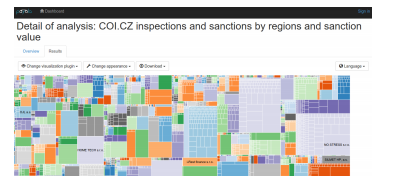
\includegraphics[width=1\textwidth]{Capture13}
\caption{Payola visualization of inspection and sanctions data’s structure using the TreeMap representation}
\end{figure}
Collaboration between users is encouraged, as visualizations and the operators used in their generation can be shared within the platform. This allows not only to re-run experiments, but to connect new analysis operators and plugins to existing pipelines in order to produce new visuals with enriched or refined data. This feature allows technical and expert users create visualizations which can later be consumed by lay users, taking away the required knowledge to collect and process data}
\subsection{ rdf:SynopsViz}
{The purpose of ref:SynopsViz  it to provide hierarchical charts and visualizations about LOD. The tool heavily relies on metadata as a means of understanding a datasets internal structure. Statistics such as total number of triples and owl:sameAs links are displayed together with the number of properties, objects,classes, languages, etc. A faceted navigation bar lets the user filter the data, which will later be visualised using bar, linea or area charts . If a area of special interest is zoomed, more fine-grained data will fill the available space.
\begin{figure}[h!]
\centering
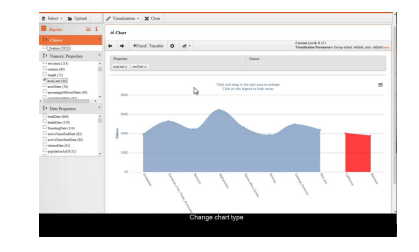
\includegraphics[width=1\textwidth]{Capture14}
\caption{rdf:SynopsViz’s faceted browsing feature over DBpedia}
\end{figure}
Even though its suitability to perform the “Overview first, zoom and filter” data visualization tasks, more advanced visualizations and interactions are missed in order to get a real feel on the underlying data. A good point though, is the possibility to obtain computed statistics about the data being queried, such as: mean, variance, minimum and maximum values, etc.}}
\subsection{Sgvizler}
{Sgvizler  is a JavaScript (JS) wrapper to visualise the result of SPARQL queries within the HTML elements of a website. To accomplish this goal, Sgvizler makes use of HTML5’s data- prefixed element attributes, where technical users can specify the
SPARQL query to perform together with the endpoint it is addressed to, the type of visualization to generate (e.g., map, treemap, bar chart, etc.), the dimensions of the chart and the format of the data. The tool works excellent with JSON (JavaScript Object Notation) formats, as the data sharing with visualization libraries is trivial (web-browser based visualization libraries are developed in JS, whose understanding of JSON is direct). Support for Google Charts7 and d3js’ 8 force directed graphs are built in.
Sgvizler adds Cross-Origin Resource Sharing (CORS)  support, in order to query SPARQL endpoints in an external domain. It requires the SPARQL endpoint to be CORS-enabled, otherwise they would not return
any information to be rendered. However, Sgvizler requires the user to have a previous SW knowledge, specially about the SPARQL querying language to write down the SELECT statements to retrieve data from the endpoint. This makes Sgvizler a good tool for expert users with semantic knowledge and with liberty to modify the HTML of the website to include the special mark-up (Figure ..). Lay users, on the other hands, may not be able to gain any benefit from the use of Sgvizler rather than the visualization of the final output.
\begin{figure}[h!]
\centering
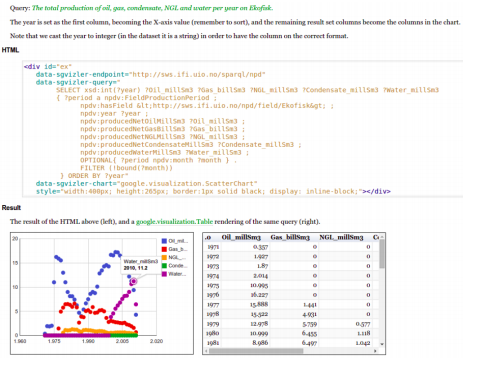
\includegraphics[width=1\textwidth]{Capture15}
\caption{Visualization example using Sgvizler, showing the HTML mark-up with the SPARQL query, the data obtained from the selection in tabular format, and the visual output on a scatter plot}
\end{figure}
}
\subsection{Visualbox}
{Taking a similar approach to Sgvizler, Visualbox  requires users to have a certain technological background, some concepts about RDF and knowledge of the SPARQL language. This tool joins different features in a single platform: SPARQL syntax highlighting to detect common errors, connection to endpoints to perform queries and control of the visualization representation through templates. Figure 8 shows the visual editor of Visualbox: the textareas allow to specify the SPARQL query to retrieve data, and how they are going to be rendered using a special templating language. The options on the sidebar filter elements to generate the final visualization, as depicted on the right side. Visualbox relies on LODSPeaKr, a framework to create LOD-based applications, setting the focus on visualizing data.
\begin{figure}[h!]
\centering
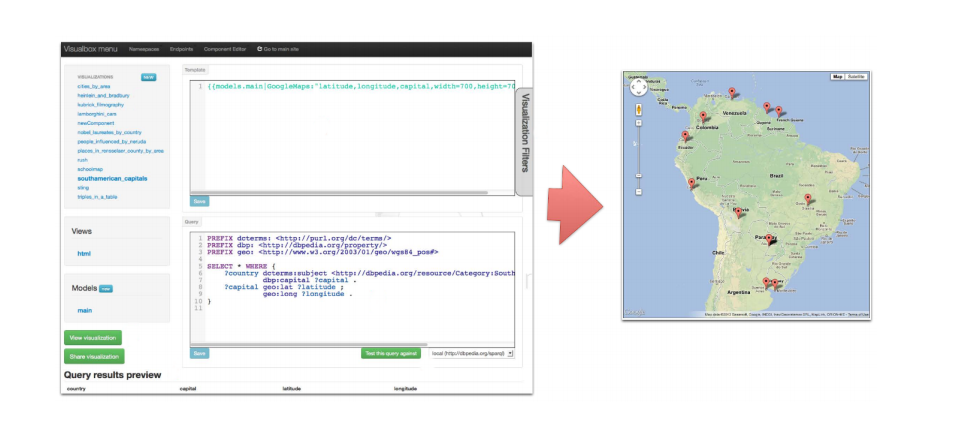
\includegraphics[width=1\textwidth]{Capture16}
\caption{Visualbox’s graphical editor and final visualization schema}
\end{figure}
Visualbox uses a templating engine similar to django’s10 where specially marked elements in the template are substituted by the values returned after performing the SPARQL query. This variables are used in the supported web-based visualization engines to create the
graphics. Collaboration between visualizers is encouraged, as all graphs are shareable through a unique URI and the charts can be downloaded as an image to be included in any document
}
\subsection{VizBoard}
{VizBoard  is a SW visualization tool build on top of the CRUISe platform , designed as a workbench for information visualization purposes. VizBoard acts as a mash-up tool, where users are able to combine different dimensions of the data to create
insightful visualizations that allow any user understand the whole picture of the dataset. Figure 4.9 displays for data panels with different representations of the underlying data. Actions performed in each panel update the
data on the rest.Interaction is heavily based on facet navigation, thus letting users select the data components most relevant for their analyses, and keep the non-desired data out of the picture. Through facets understanding the principal
components the data is categorised in is quite straight. Finally, VizBoard supports all the information about visualization rendering using The Visualization Ontology (VISO) , a multi-model vocabulary which describes all the concepts and relations on the graphics
and visualization fields.
\begin{figure}[h!]
\centering
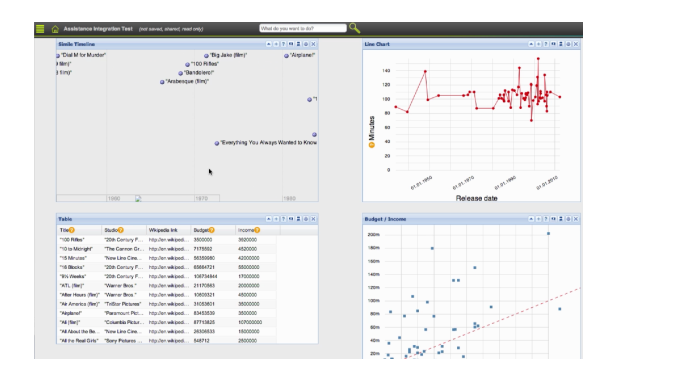
\includegraphics[width=1\textwidth]{Capture17}
\caption{Data panels on VizBoard demo}
\end{figure}
}
\section{Linked Data Visualization Model}
{In this section we present the Linked Data Visualization Model (LDVM), which is based on a preliminary version . First, we give an overview of the model and then we formalize its key elements. We also provide examples to explain the principles}
\subsection{Overview of LDVM}
{We use the Data State Reference Model (DSRM) proposed by Chi  as a conceptual framework for our Linked Data Visualization Model (LDVM). DSRM describes the visualization process in a generic way. Our LDVM is an adaptation of this generic model
for the specifics of the visualization of RDF and Linked Data. The main difference is that in certain parts, LDVM works solely with RDF data model for increased automation while DSRM is generic in each of its parts and does not constraint the applied data
models. We also extend DSRM with three additional concepts – analyzers, transformers and visualizers. They denote reusable software components that can be chained to form an LDVM instance. Figure. shows an overview of the LDVM. The names of the
stages, transformations and operators proposed by DSRM have been slightly adapted to the context of RDF and Linked Data. LDVM resembles a pipeline starting with raw source data (not necessarily RDF) and results with a visualization of the source data. It
is organized into four stages that source data needs to pass through:
\begin{enumerate}
\item{Source RDF and non-RDF data: raw data that can be RDF or adhering to other data models and formats (e.g. XML, CSV) as well as semi-structured or even nonstructured data (e.g. HTML pages or raw text)}
\item{Analytical abstraction: extraction and representation of relevant data in RDF obtained from source data}
\item{Visualization abstraction: preparation of an RDF data structure required by a particular visualization technique; the data structure is based on generic data types for visual analysis proposed by Shneiderman [14] (i.e., 1D, 2D, 3D or multi-dimensional
data, temporal data (as a special case of 1D), tree data, or network data) }
\item{View: creation of a visualization for the end user}
\end{enumerate}
\begin{figure}[h!]
\centering
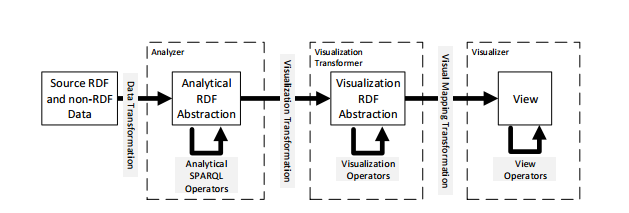
\includegraphics[width=1\textwidth]{Capture18}
\caption{High level LDVM overview}
\end{figure}
}
Data is propagated through the LDVM pipeline from one stage to another by applying three types of transformation operators:
\begin{enumerate}
\item{Data transformation: transforms the raw data represented in a source data model or format into a representation in the RDF data model; the result forms the base for creating the analytical RDF abstraction}
\item{Visualization transformation: transforms the obtained analytical abstraction into a visualization abstraction}
\item{Visual mapping transformation: maps the visualization abstraction data structure to a concrete visual structure on the screen using a particular visualization technique specified using a set of parameters. }
\end{enumerate}
There are operators within the stages that allow for in-stage data transformations:
\begin{enumerate}
\item{Analytical SPARQL operators: transform the output of the data transformation to the final analytical abstraction (e.g. aggregations, enrichment from LOD)}
\item{Visualization operators: further refine the visualization abstraction data structure (e.g., its condensation if it is too large for transparent visualization).}
\item{View operators: allow a user to interact with the view (e.g., rotate, scale, zoom, etc.). }
\end{enumerate}
}
\subsection{LDVM stages}
{Source RDF and non-RDF Data Stage. The first stage considers RDF as well as nonRDF data sources as many data sources are currently not RDF. The data transformation transforms the source data to an RDF representation that forms a base for creating an
analytical abstraction. If the source RDF data does not have a suitable structure for the following analysis, the transformation can be a sequence of one or more SPARQL queries that map the source data to the required structure. Since data extraction is a vast research field on its own.\\
Analytical RDF Abstraction Stage. The output of the second stage (analytical RDF abstraction) is produced by applying a sequence of various in-stage analytical SPARQL
operators on the RDF output produced by the data transformation. We call the sequence an analyzer . Our goal is to enable users to reuse existing analyzers (possibly created by other users) for analyzing various datasets. We want to enable users
to find analyzers that can be applied for analyzing a given data set and, vice versa, to find datasets that may be analyzed by a given analyzer automatically. Therefore, it is necessary to be able to decide whether an analyzer can be applied on a given dataset, i.e. whether the analyzer is compatible with the dataset.\\
Visualization Abstraction Stage. An analytical abstraction is not a suitable data structure for visualization. We want to ensure that a visualization tool is reusable for
different analytical abstractions. Building specific visualizers for particular analytical abstractions would not enable such reuse. This is because each visualization tool visualizes particular generic characteristics captured by the analytical abstraction. For
example, there can be a tool that visualizes tree structures using the TreeMap technique or another tool that visualizes the same structures using the SunBurst technique. And, another tool may visualize 2-dimensional structures on Google Maps. An analytical abstraction may contain encoded both tree structure as well as 2-dimensional structure. All three mentioned tools can be applied to the analytical abstraction as well as on any other abstraction which contains the same structures encoded. Therefore, we
need to transform the analytical abstraction into a more generic data structure based on Generic Visualization Data Types (GVDTs), listed in Table 4.1. The GVDTs are inspired by Shneiderman data types. This structure is then what is visualized by visualization tools. This transformation is performed by the visualization abstraction stage of LDVM. Its output (visualization abstraction) is produced by a component that performs visualization transformation followed by a set of in-stage visualization operators. We call it a visualization transformer.
\begin{table}
\begin{center}
\begin{tabular}{|l|c|r|}
\hline
RDF Vocabulary & Data Type & Visualization Tool\\
\hline
xsd:int, dc:subject,... (count)  & 1D & Histogram \\
\hline
wgs84:lat, geo:point,...& 2D & Map\\
\hline
visko:3DPointPlot,...& 3D & 3D Rendering\\
\hline
qb:Observation, scovo:Item,...&Multidimensional&Chart\\
\hline
xsd:date, ical:dtstart,...&Temporal&Timeline, Calendar,...\\
\hline
rdfs:subClassOf, skos:narrower,...&Tree&Treemap, SunBurst,...\\
\hline
foaf:knows,...&Network&Graph,...\\
\hline
\end{tabular}
\end{center}
\caption{Generic visualization data types}
\end{table}
 }\\ \\
\textbf{\large Conclusion}\\ \\
{We presented in this chapter the frequent approches of linked data visualization as well as the linked data visualization model.At the end of this chapter we can choose the most efficient visualization technique in our case which is SGvizler and this choise will be explained in details in the final chapter that presents the practical part of this work such as data transformation to RDF form ,the  writing of the SPARQL queries and the development of the user interface.}
\chapter {Data processing and User Interface Development }
\textbf{\large Introduction }\\ \\
{We present in this final chapter all the steps of the project realization with the details of the used technologies.This chapter is divided in two important parts , the first one is for the data transformation and the second one is for the development of the web application.}
\section {Datasets selection }
{As mentioned in chapter 3 , there are many interesting open datasets available on the web. In our project we are interested  in Belgium data especially  the data related to crimes , population and external immigration .Thus we selected three datasets ;the population , the external immigration and the number of crimes in Belgium from 2000 to 2013 , and our data sources are the open government data of Belgium ( \url {http://data.gov.be/fr})  and the european portal (\url {http://www.europeandataportal.eu/}).
The next figures show somes samples of the gathered data.
\begin{figure}[ht]
\centering
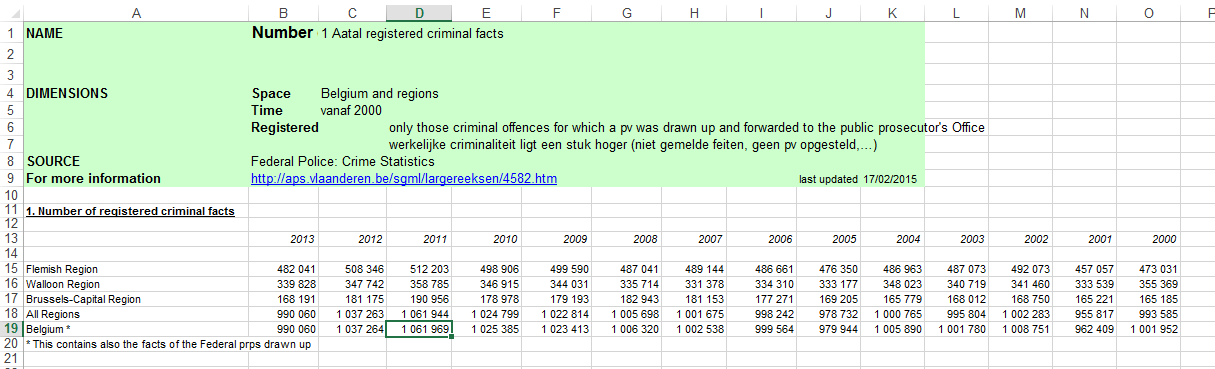
\includegraphics[width=1\textwidth]{cap1}
\caption{Number of Registred crimes in Belgium}
\end{figure}
\begin{figure}[ht]
\centering
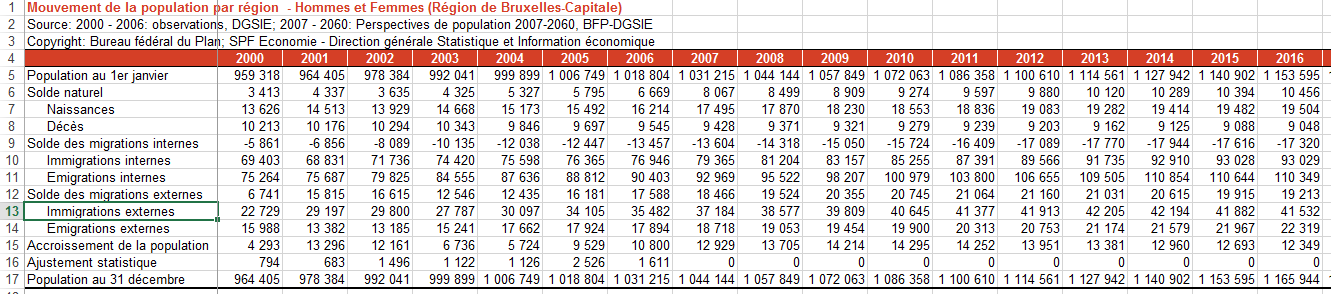
\includegraphics[width=1\textwidth]{cap2}
\caption{Population movement in Belgium}
\end{figure}
\begin{figure}[ht]
\centering
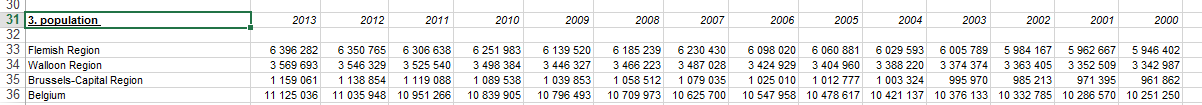
\includegraphics[width=1\textwidth]{cap3}
\caption{ Belgium population}
\end{figure} }
\section { Data conversion to RDF }
\subsection {Ontologies definition }
{In order to convert our raw data into linked data , we have to define at first   our RDF graph and then we define the required ontologies according to it. The next figure present the RDF graph that we have defined
\begin{figure}[ht]
\centering
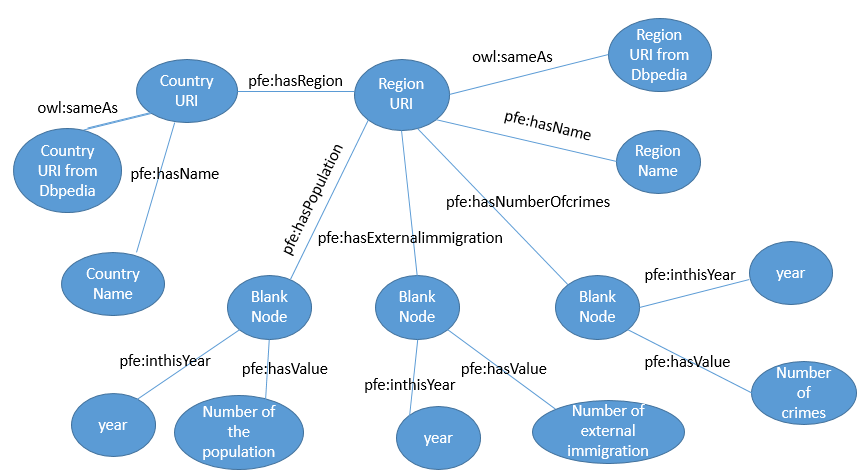
\includegraphics[width=1\textwidth]{Capture77}
\caption{ RDF graph}
\end{figure}
}


\bibliographystyle{plain}
\bibliography{references.bib}
\nocite{*}
\appendix


\section{Source Code}

\begin{lstlisting}
  print('Hello World!')
     use indentation and {special &characters}
\end{lstlisting}





\end{document}
